\documentclass{article}
\usepackage[utf8]{inputenc}
\usepackage{geometry}
\usepackage{amsmath}
\usepackage{url}
\usepackage[utopia]{mathdesign}
\usepackage{lipsum}  
\usepackage{lmodern}
\usepackage{listings}
\usepackage{tikz}
\usetikzlibrary{arrows.meta, positioning}

 \geometry{
 a4paper,
 total={170mm,257mm},
 left=20mm,
 top=20mm,
 }
 \usepackage{graphicx}
 \usepackage{titling}

 \title{Report \#6}
\author{GU JUN}
 
 \usepackage{fancyhdr}
\fancypagestyle{plain}{%  the preset of fancyhdr 
    \fancyhf{} % clear all header and footer fields
%    \fancyfoot[R]{\includegraphics[width=5cm]{}}
    \fancyfoot[L]{\today}
    \fancyhead[L]{Analytical Mechanics 80848\#5}
    \fancyhead[R]{HIRAI SHINCHI}
}
\makeatletter
\renewcommand{\maketitle}{%
  \newpage
  \null
  \vskip 1em%
  \begin{center}%
  \let \footnote \thanks
    {\LARGE \@title \par}%
    \vskip 1em%
    %{\large \@date}%
  \end{center}%
  \par
  \vskip 1em}
\makeatother


\begin{document}

\maketitle

\noindent\begin{tabular}{@{}ll}
    Student & \theauthor\\
    ID number & 6132230056 \\
\end{tabular}
\section*{Dynamic Simulation of Rotation}
Simulate the rotation of a rigid cylinder in 3D space. Define class RigidBody Cylinder as a subclass of RigidBody. Use appropriate values of geometrical and physical parameters of the cylinder. Apply
torque vectors with different directions.
\section*{Class RigidBody\_Cylinder}
First, we define the class \texttt{RigidBody\_Cylinder} as a subclass of \texttt{RigidBody}. The class \texttt{RigidBody\_Cylinder} has the height and radius of the cylinder as its properties.
To calculate its inertia matrix, we use the formula for the inertia matrix of a cylinder. The inertia matrix of a cylinder is given by
\begin{equation}
    I = \frac{1}{12}m\begin{pmatrix}
    3r^2+h^2 & 0 & 0\\
    0 & 3r^2+h^2 & 0\\
    0 & 0 & 6r^2
    \end{pmatrix}
\end{equation}
where $m$ is the mass of the cylinder, calculated by $m = \rho \pi r^2 h$, $r$ is the radius of the cylinder, and $h$ is the height of the cylinder. 
With this equation, we can define our RigidBody\_Cylinder class as follows:
\begin{footnotesize}
\begin{lstlisting}[language=Matlab]
  classdef RigidBody_Cylinder < RigidBody
    properties
        r, h;
    end
    methods
        function obj = RigidBody_Cylinder (rho, r, h)
            obj@RigidBody(1,eye(3));
            m = rho*pi*r^2*h;
            Jz = (1/2)*m*r^2;
            Jx = (1/12)*m*(3*r^2 + h^2);
            Jy = Jx;
            J = diag([Jx, Jy, Jz]);
            obj = obj.mass_and_inertia_matrix(m, J);
            obj.density = rho;
            obj.r = r;
            obj.h = h;
        end
        
        function draw(obj, pos, q)
        % this function is omitted for simplicity
        end
    end
end
\end{lstlisting}
\end{footnotesize}
\newpage

\section*{Simulation Results}
We simulate the rotation of a cylinder with radius $r = 2$, height $h = 6$, and density $\rho = 1$. The external torque is defined as a function of time:
\begin{equation}
  \tau(t) = 
  \begin{cases} 
    [12, 0, 0] & \text{if } t \leq 5 \\
    [0, -12, 0] & \text{if } t > 5 \& t \leq 10 \\
    [0, 0, 0] & \text{if } t > 10
  \end{cases}
\end{equation}
The simulation results are shown in the following figures.
\begin{figure}[h!]
  \centering
  \begin{tabular}{cc}
    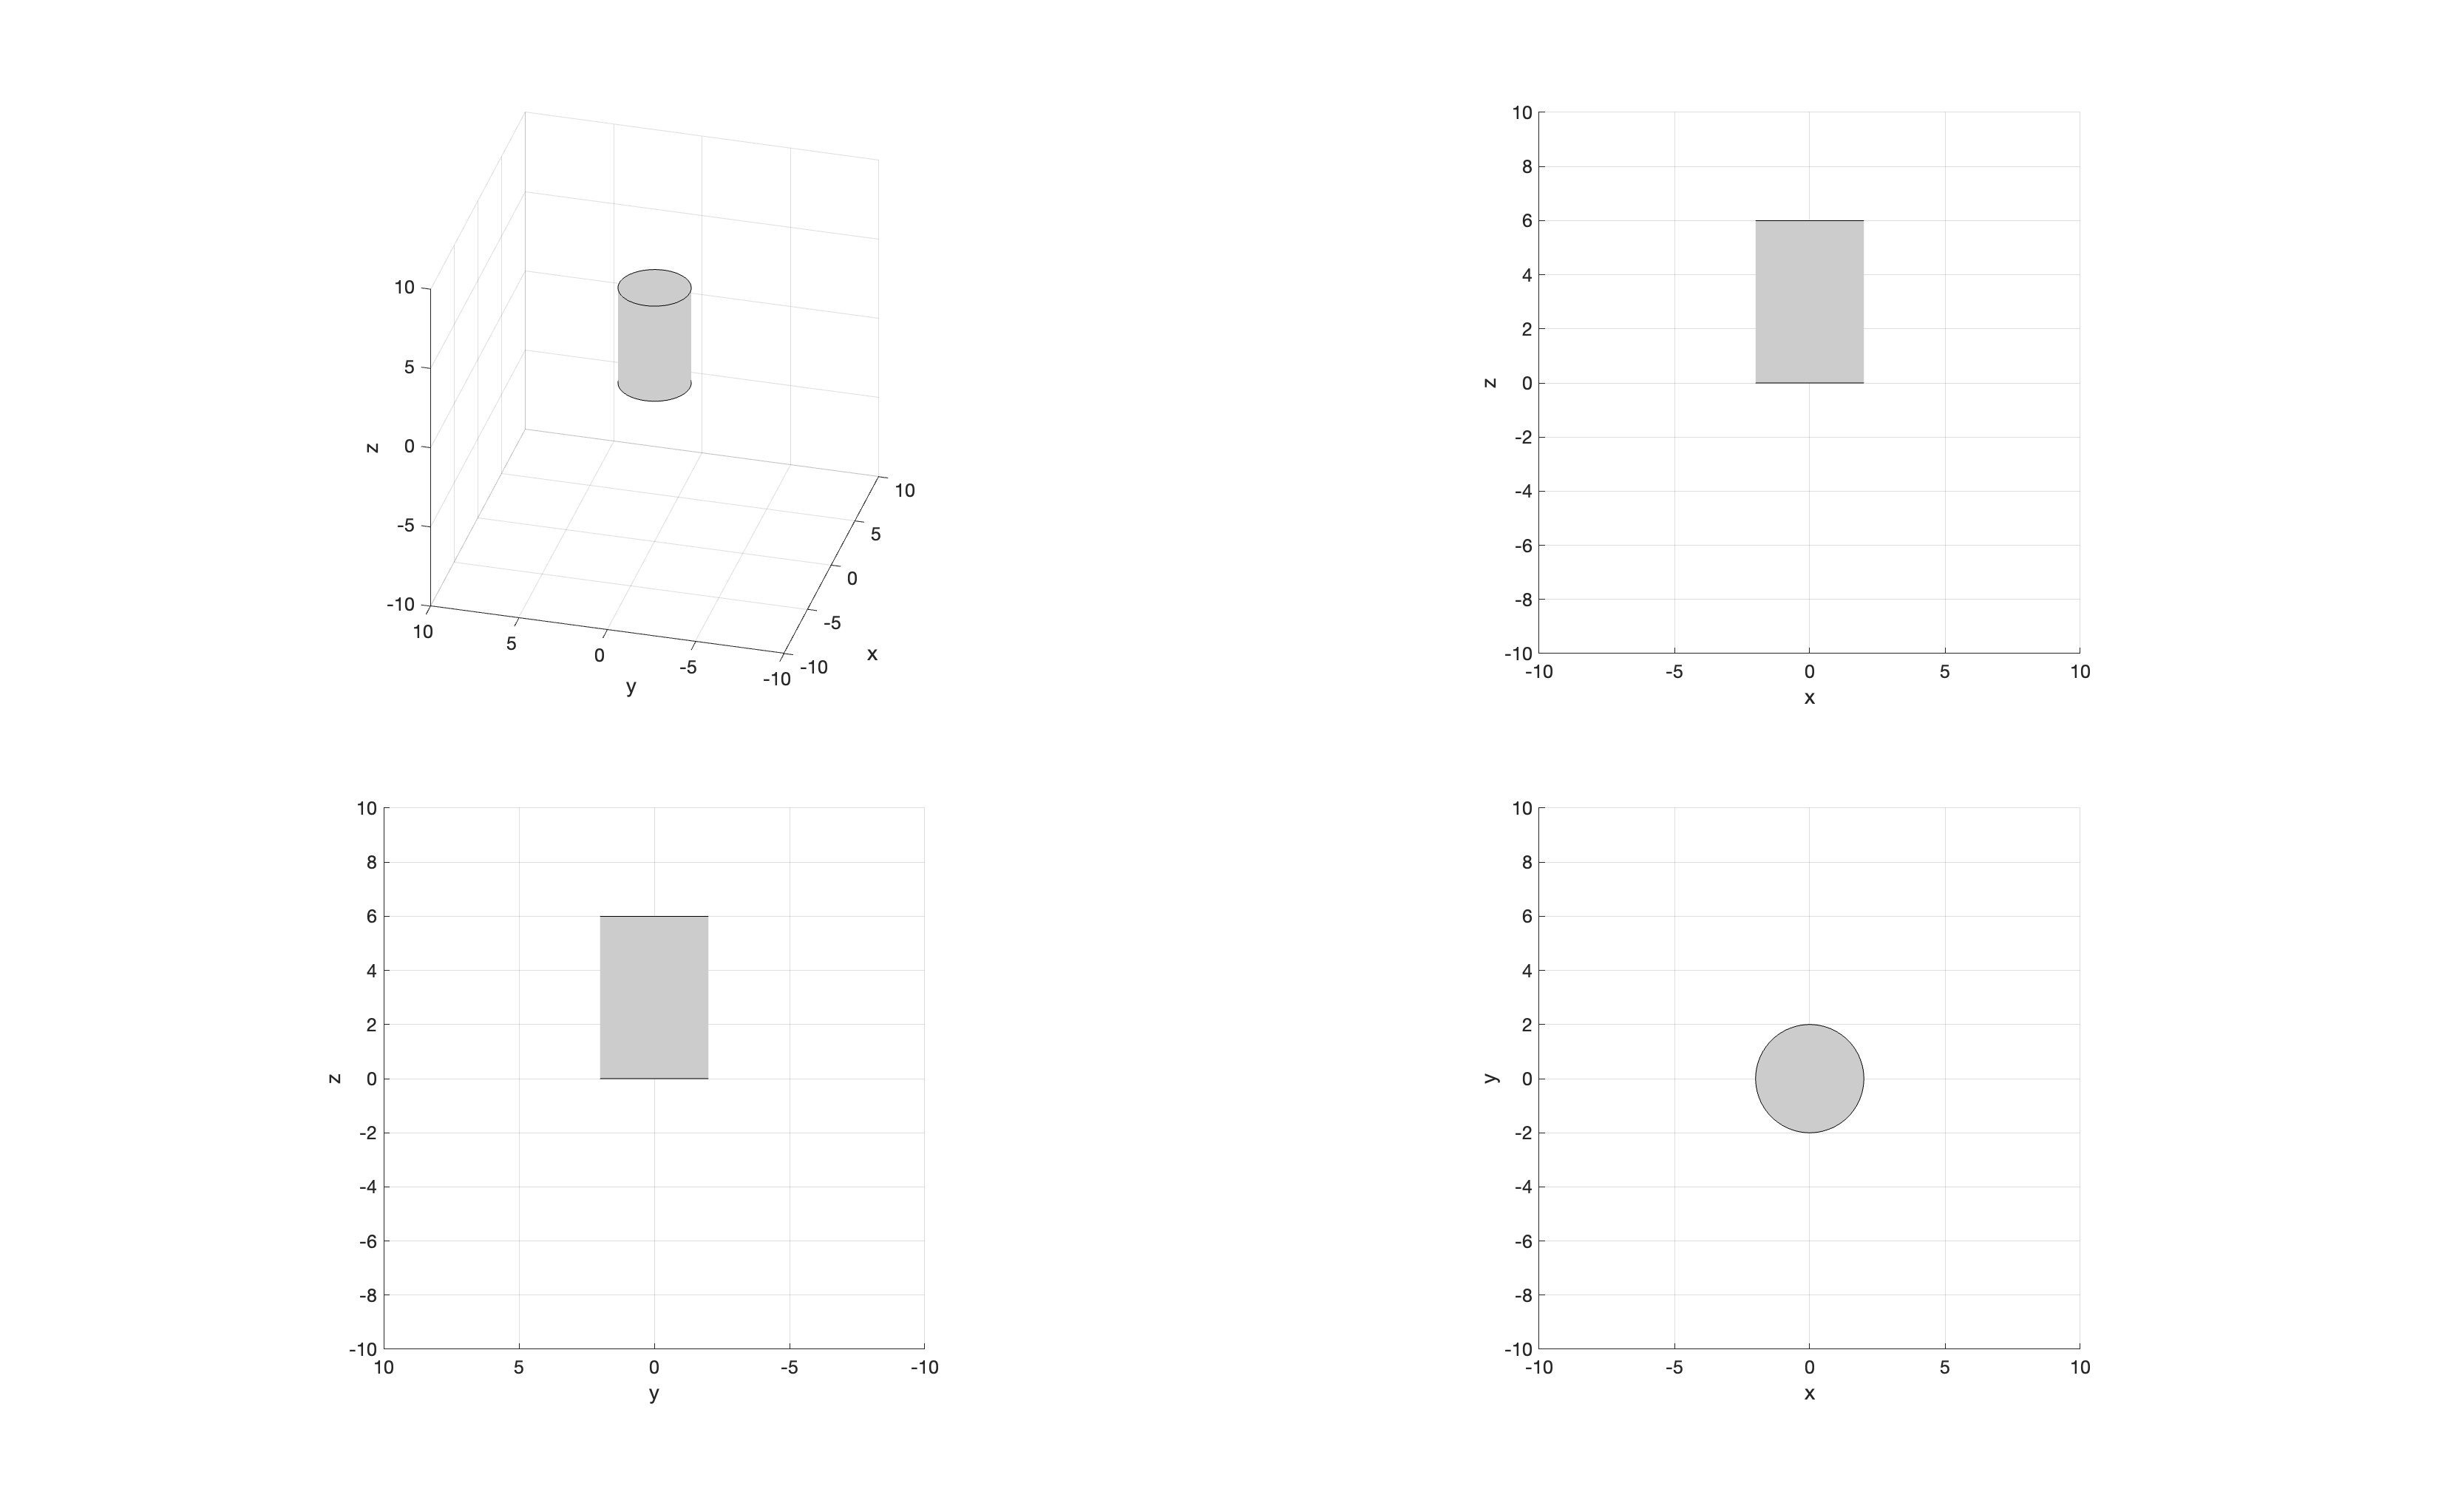
\includegraphics[width=0.45\textwidth]{assets/figure_0.png} & 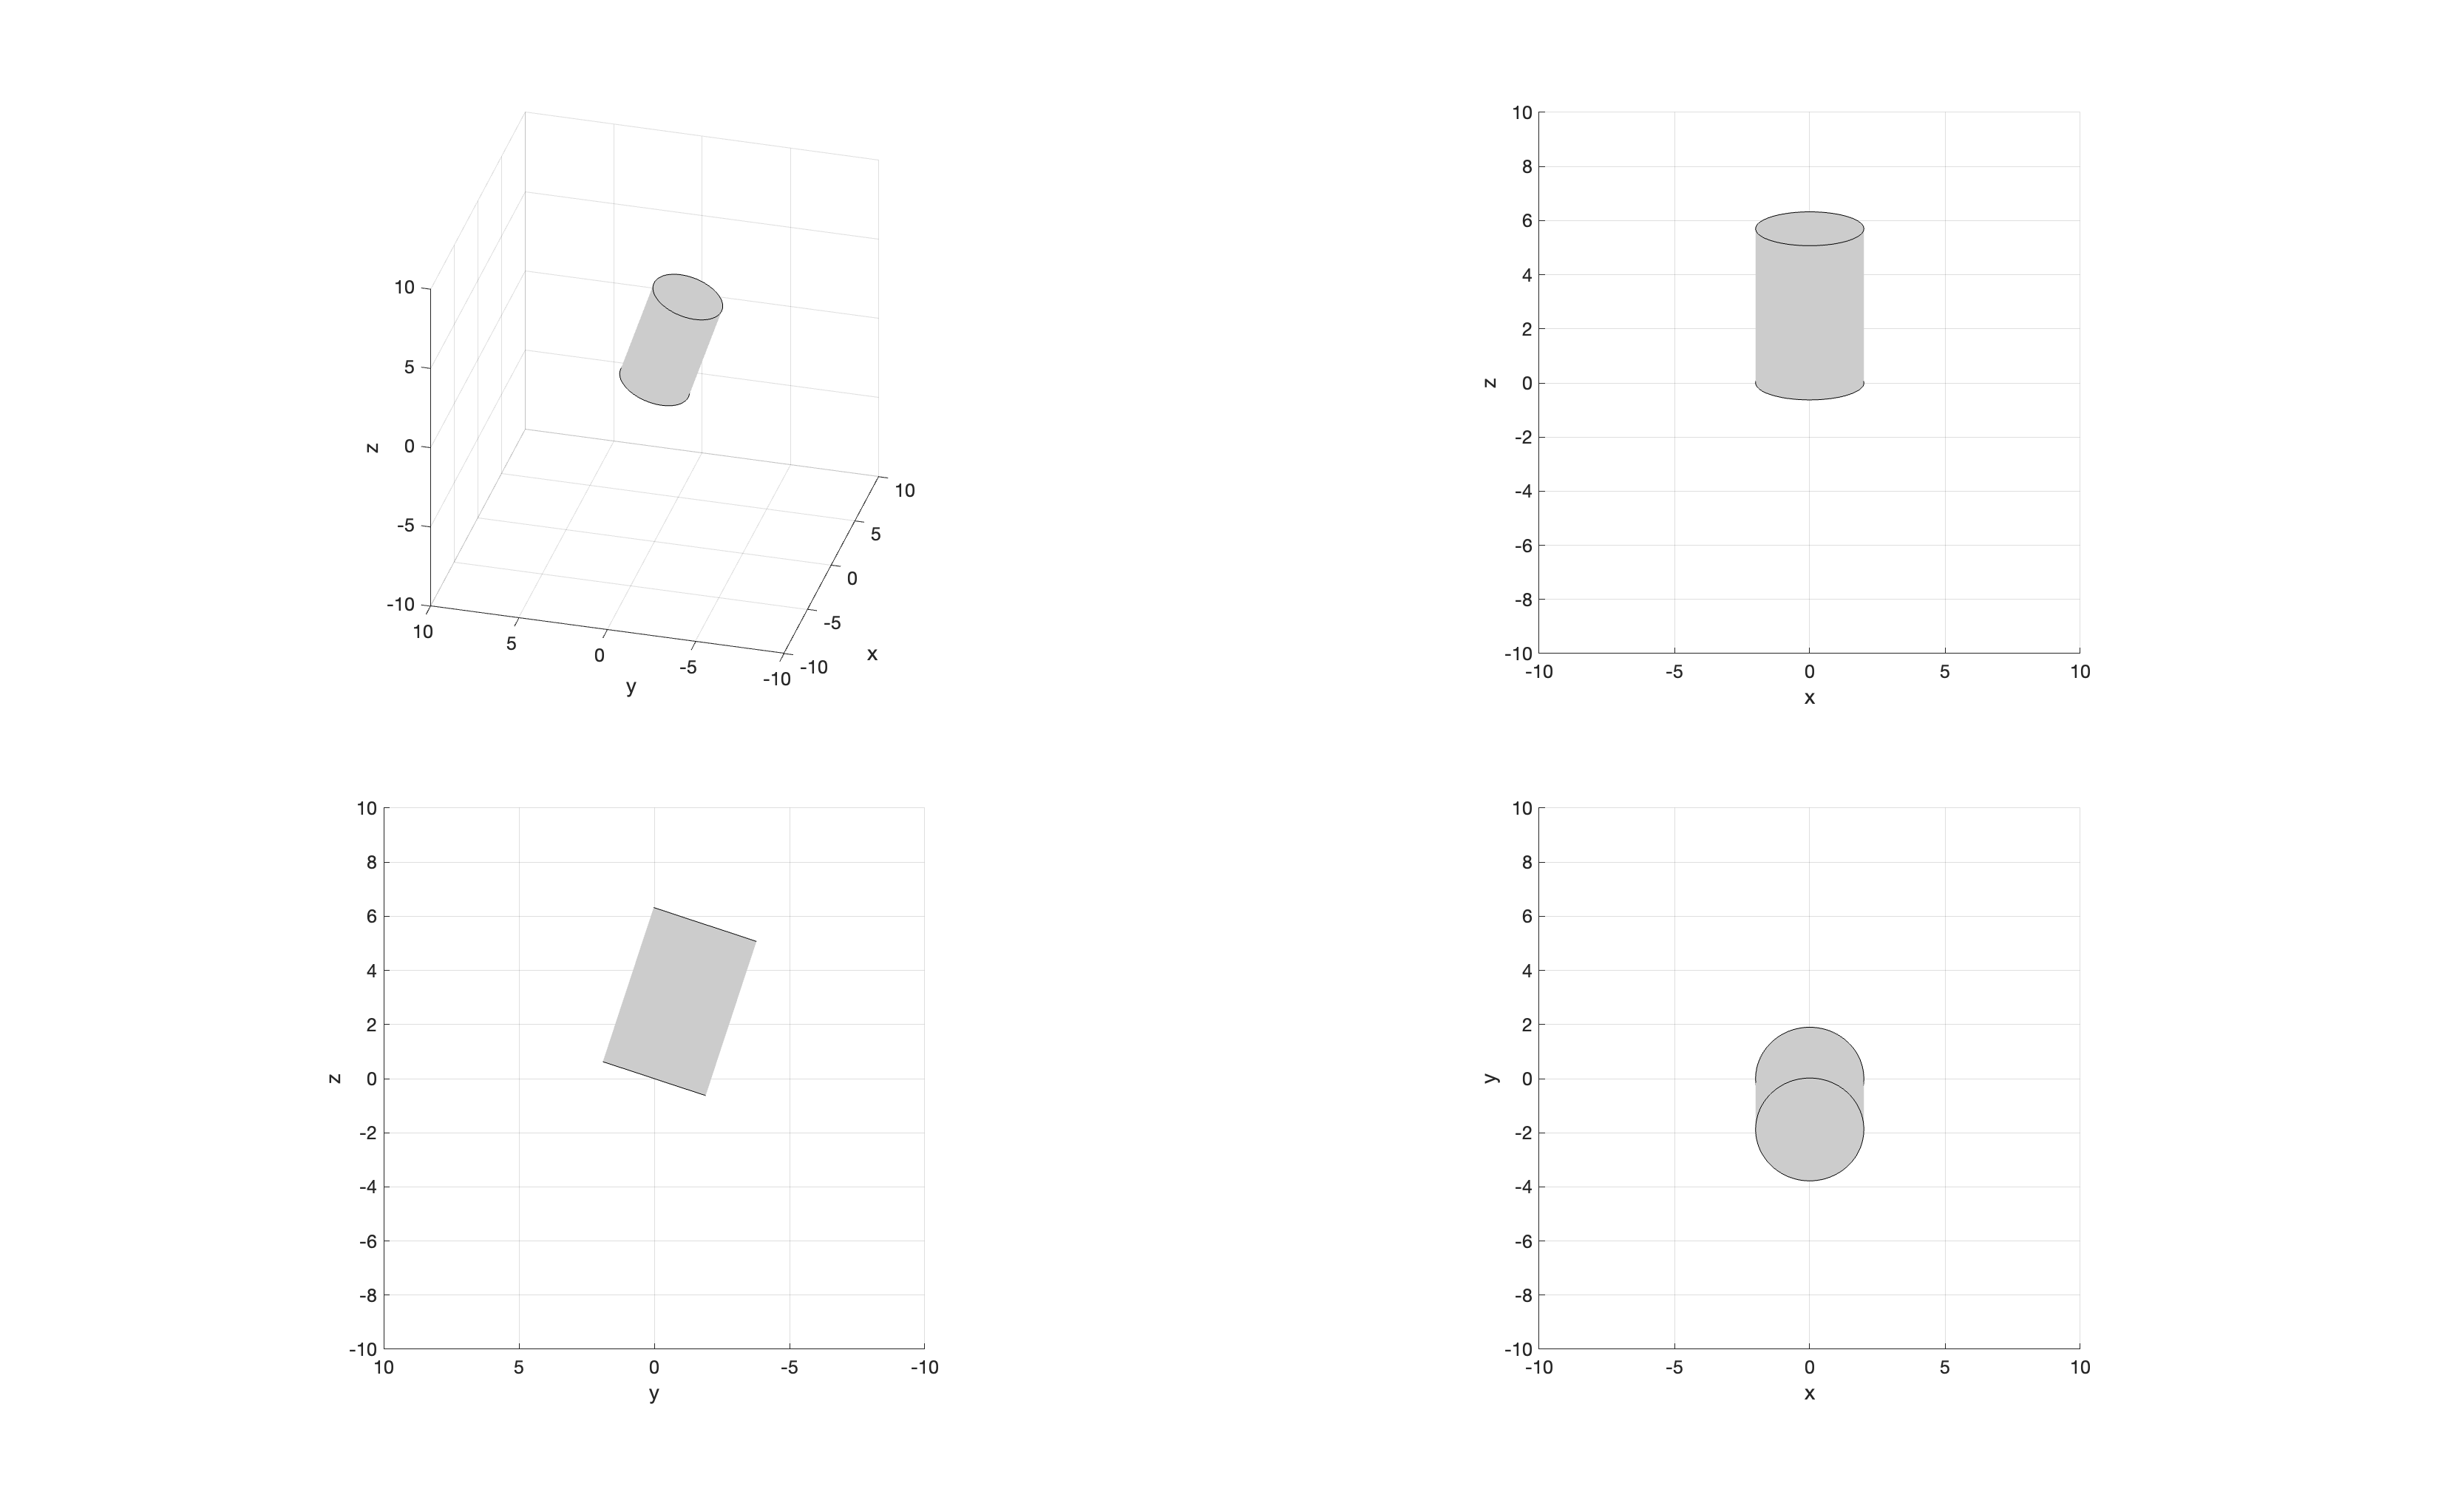
\includegraphics[width=0.45\textwidth]{assets/figure_4.png} \\
    (a) $t = 0$ & (b) $t = 4$ \\
    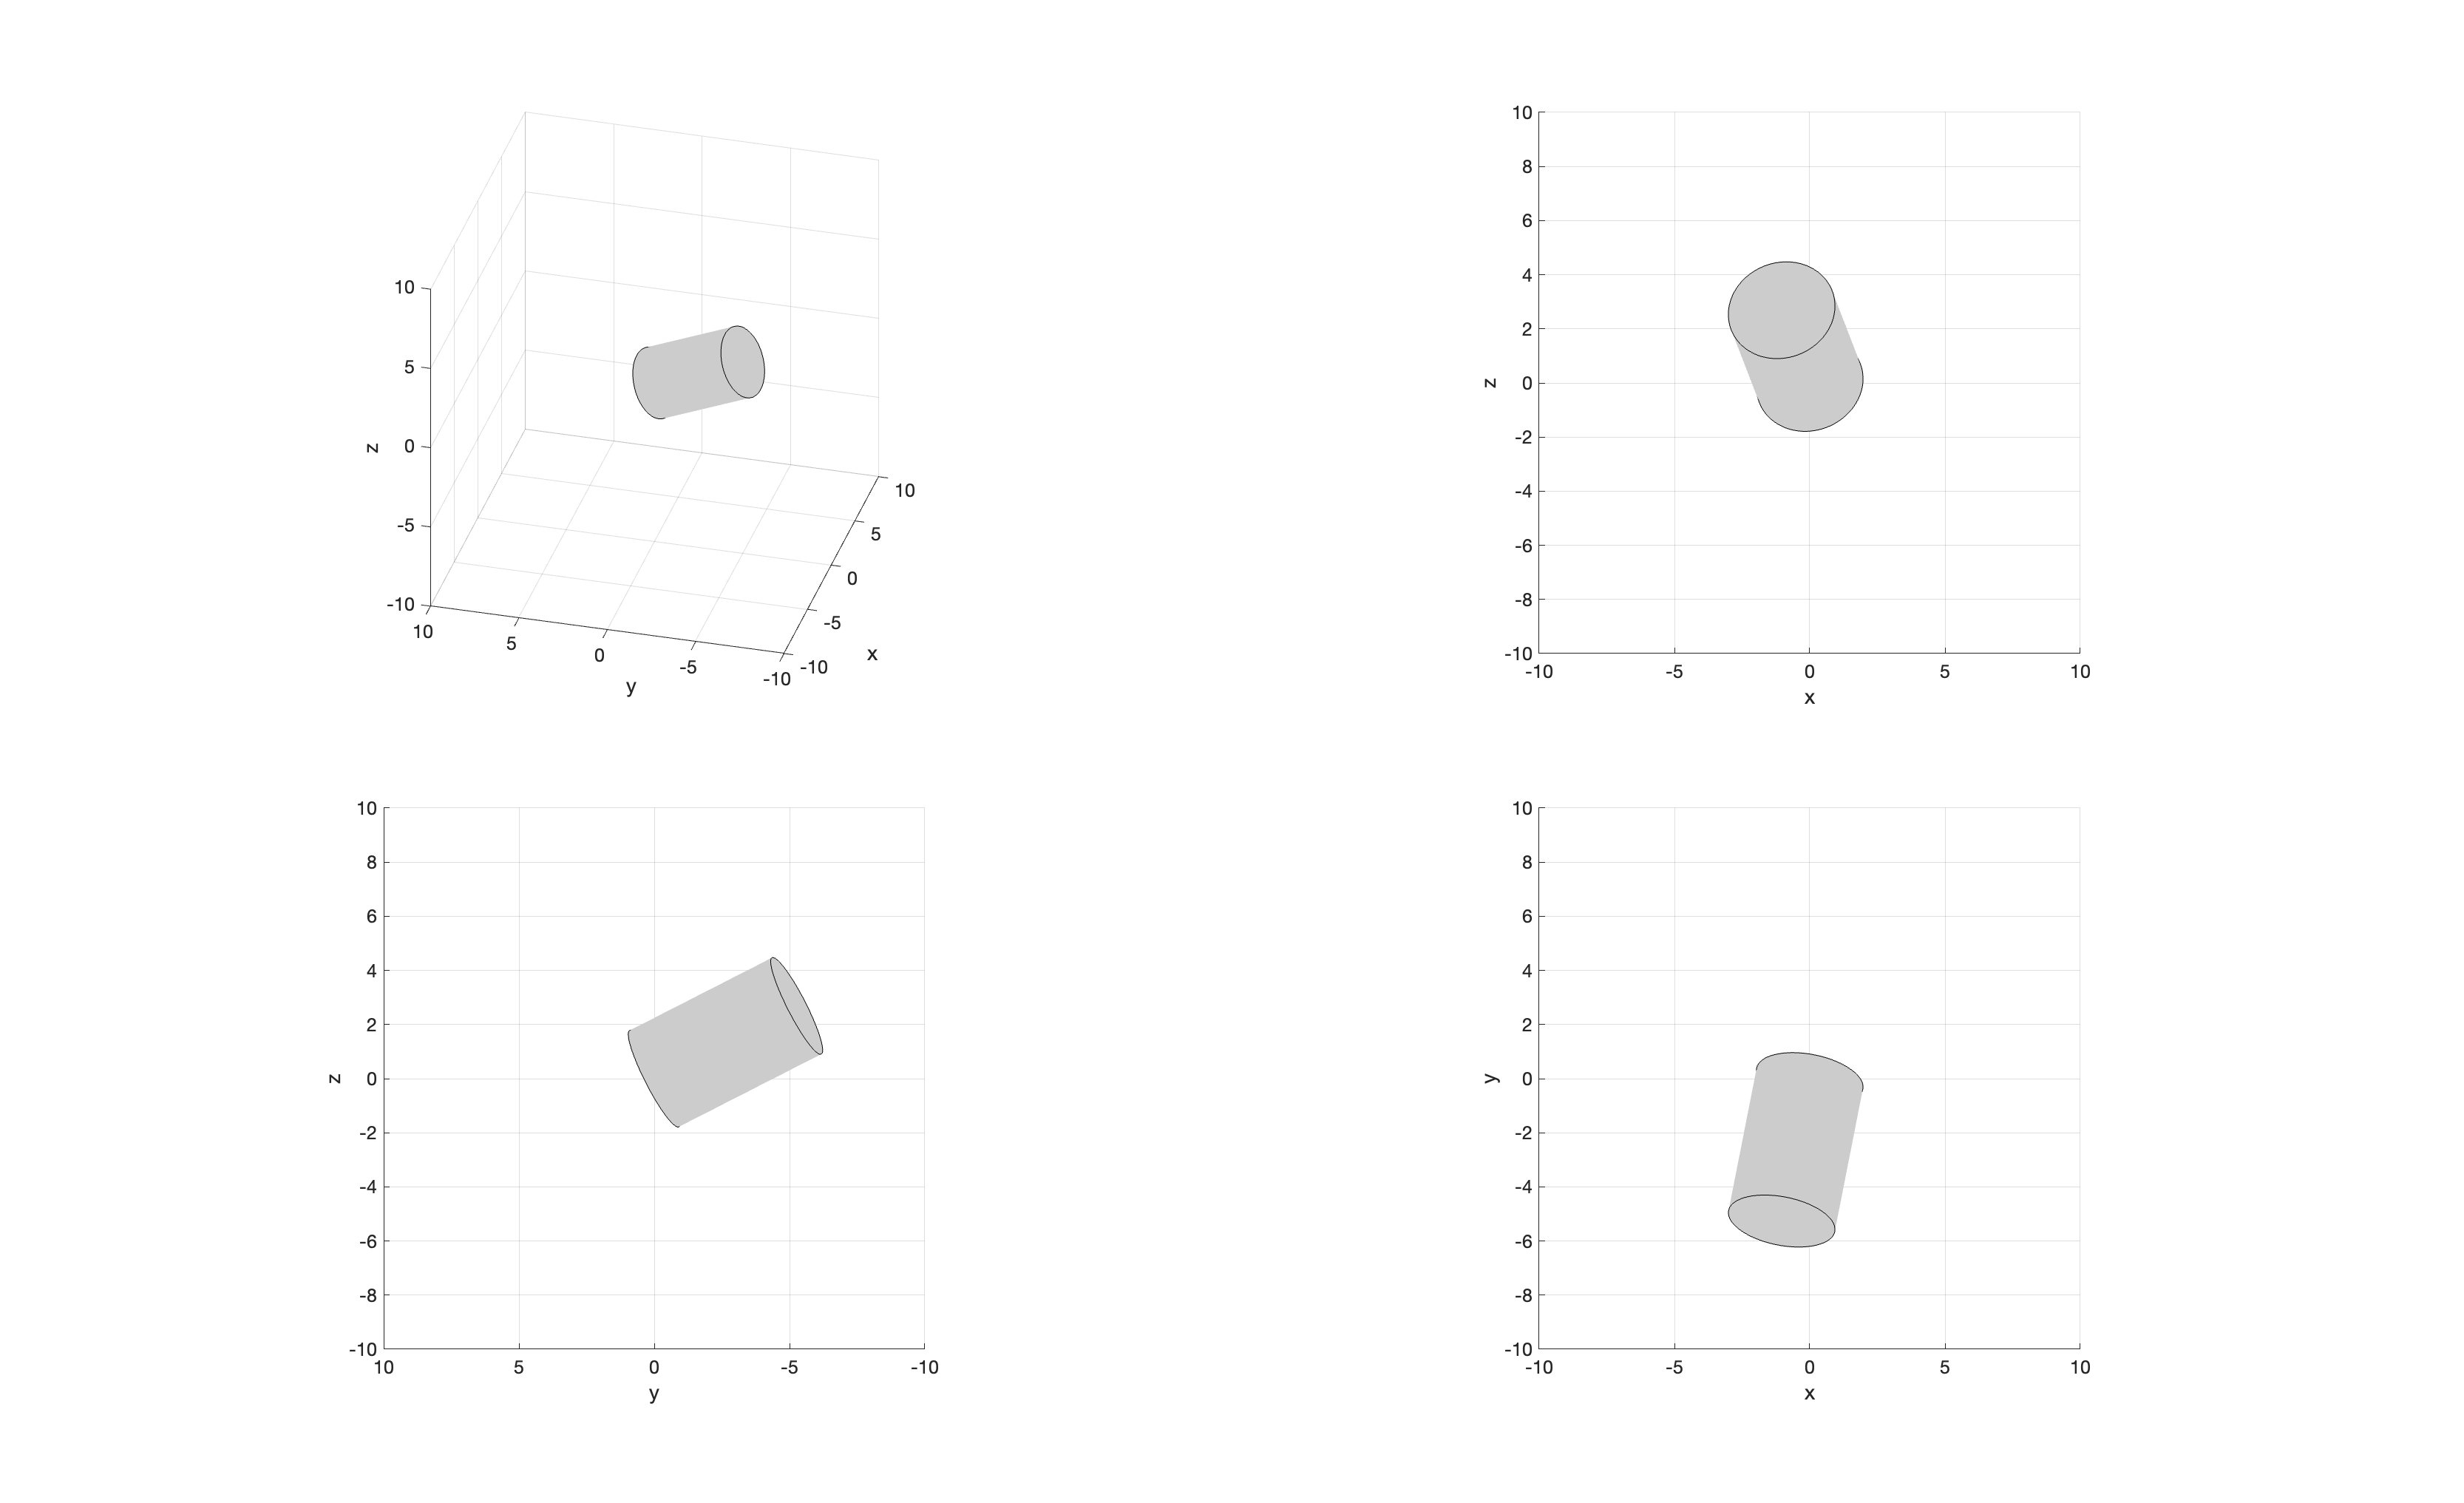
\includegraphics[width=0.45\textwidth]{assets/figure_8.png} & 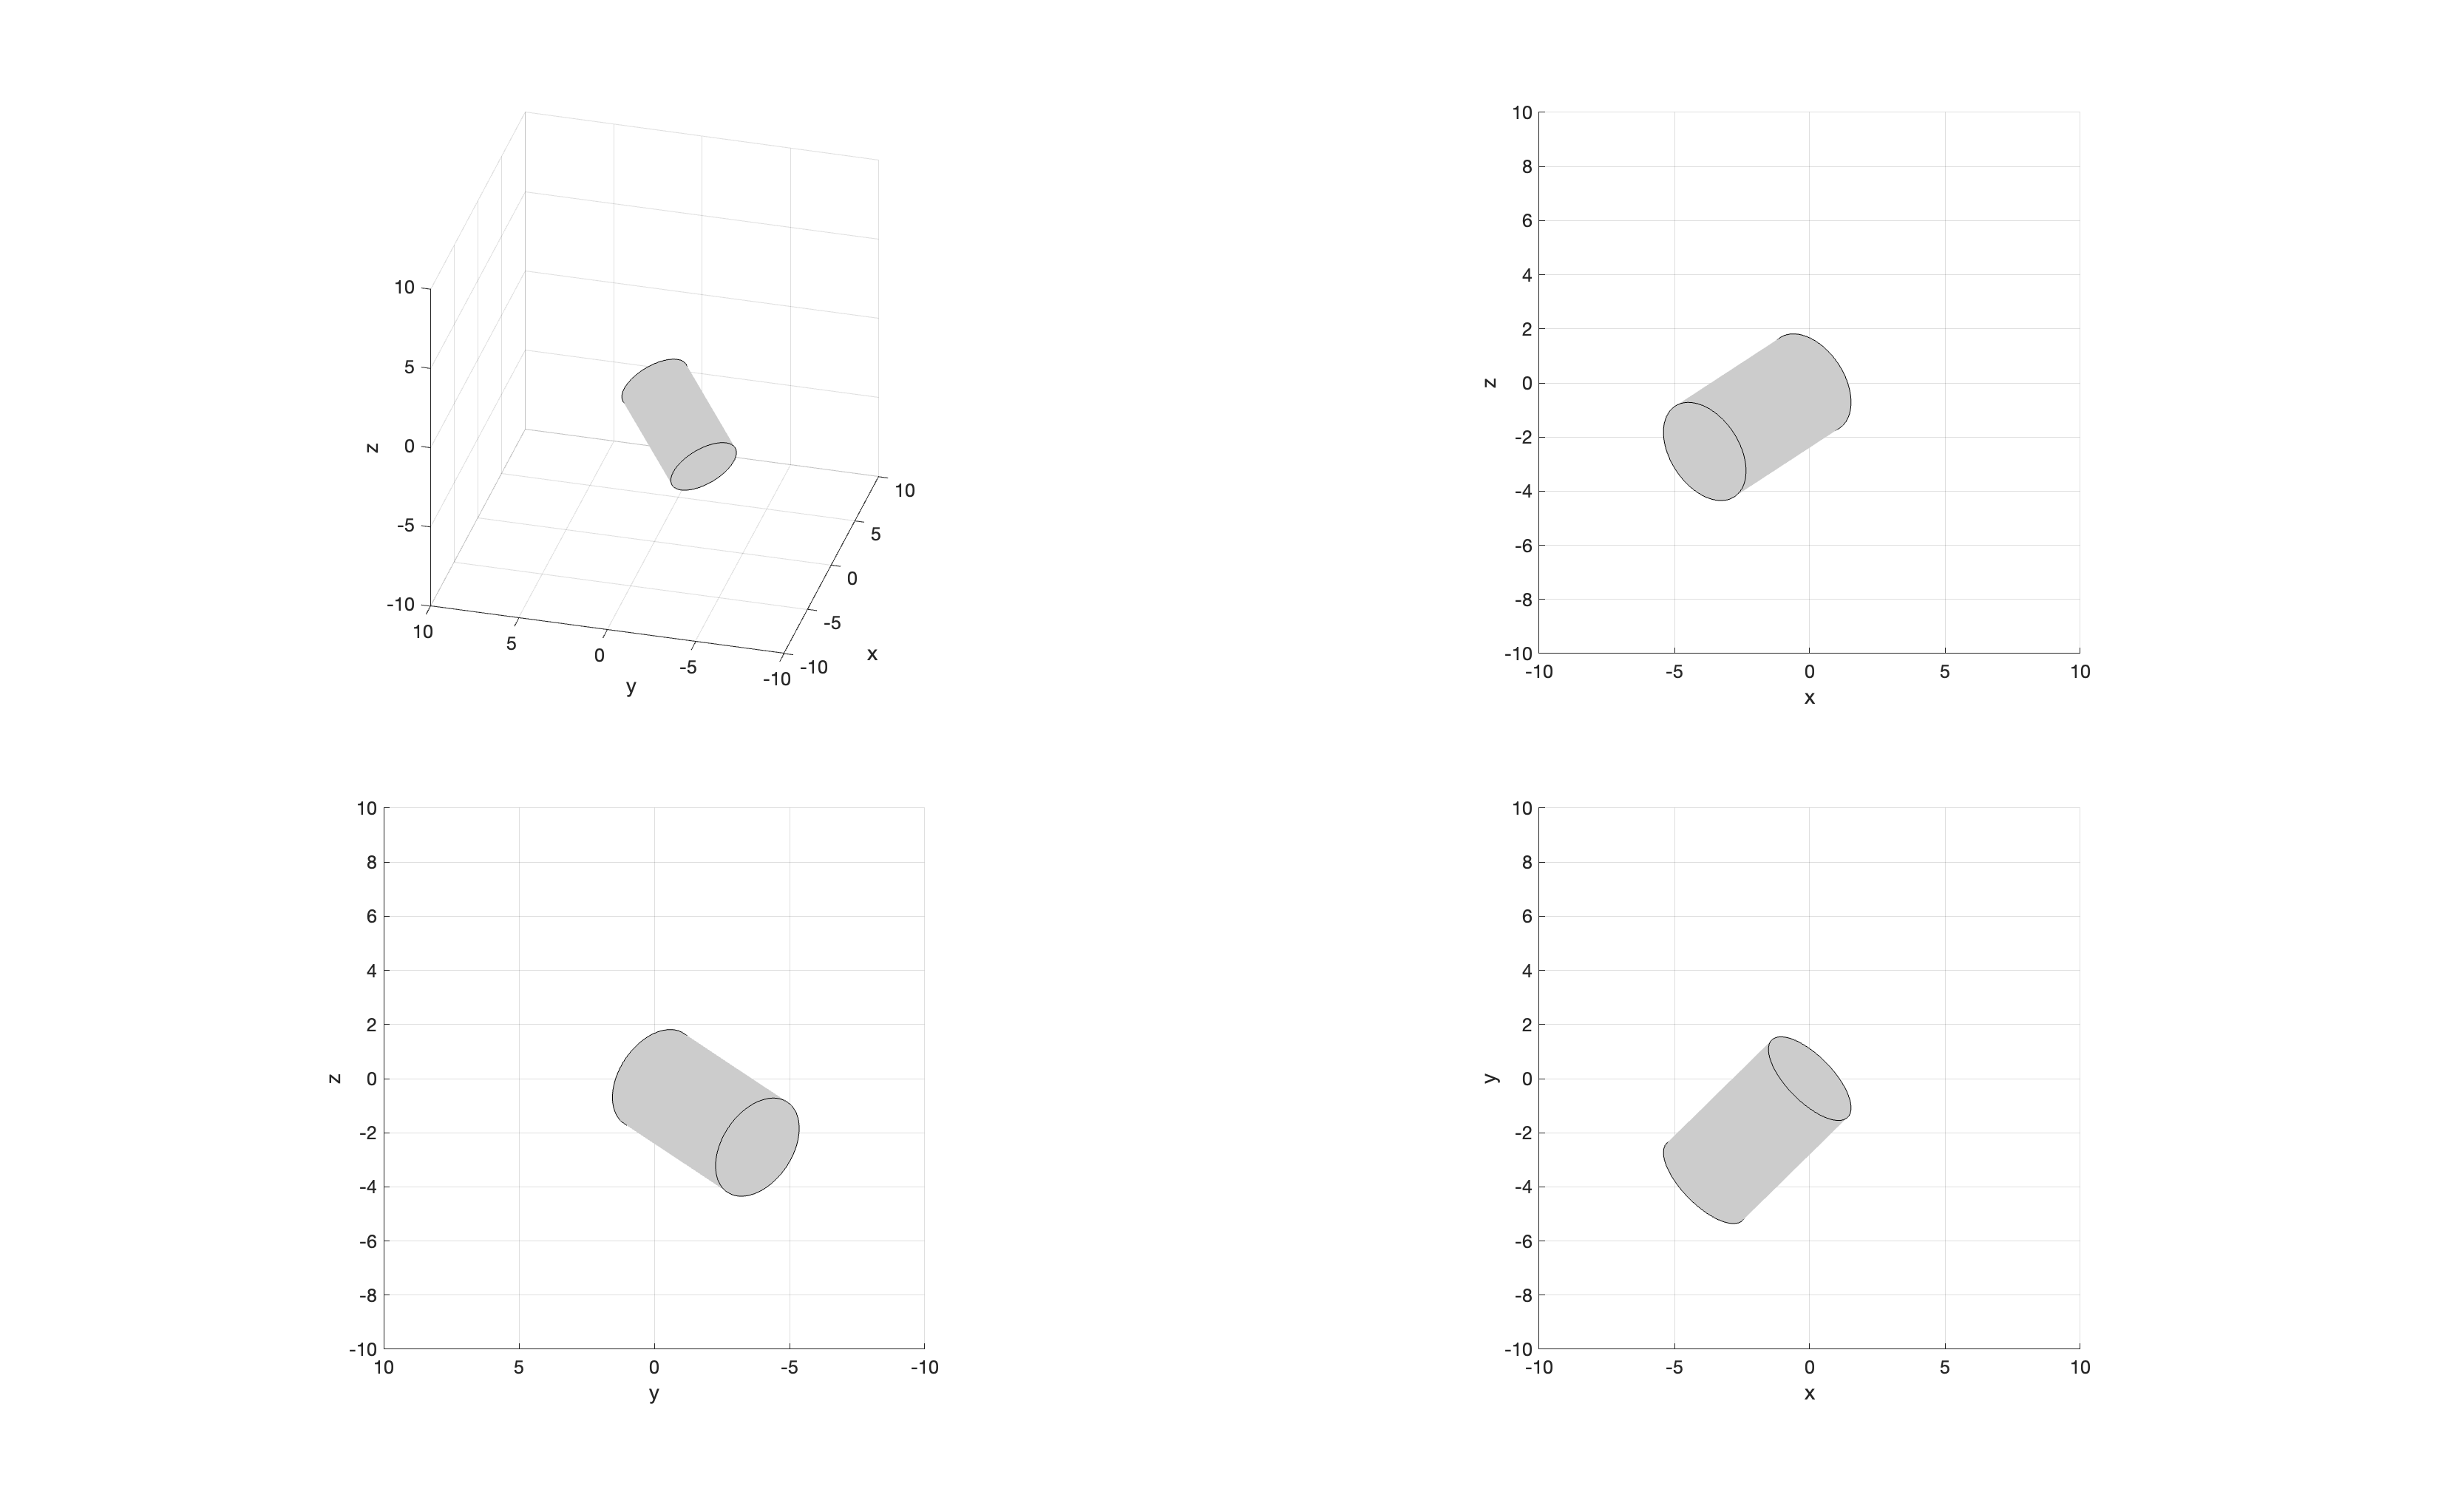
\includegraphics[width=0.45\textwidth]{assets/figure_12.png} \\
    (c) $t = 8$ & (d) $t = 12$ \\
    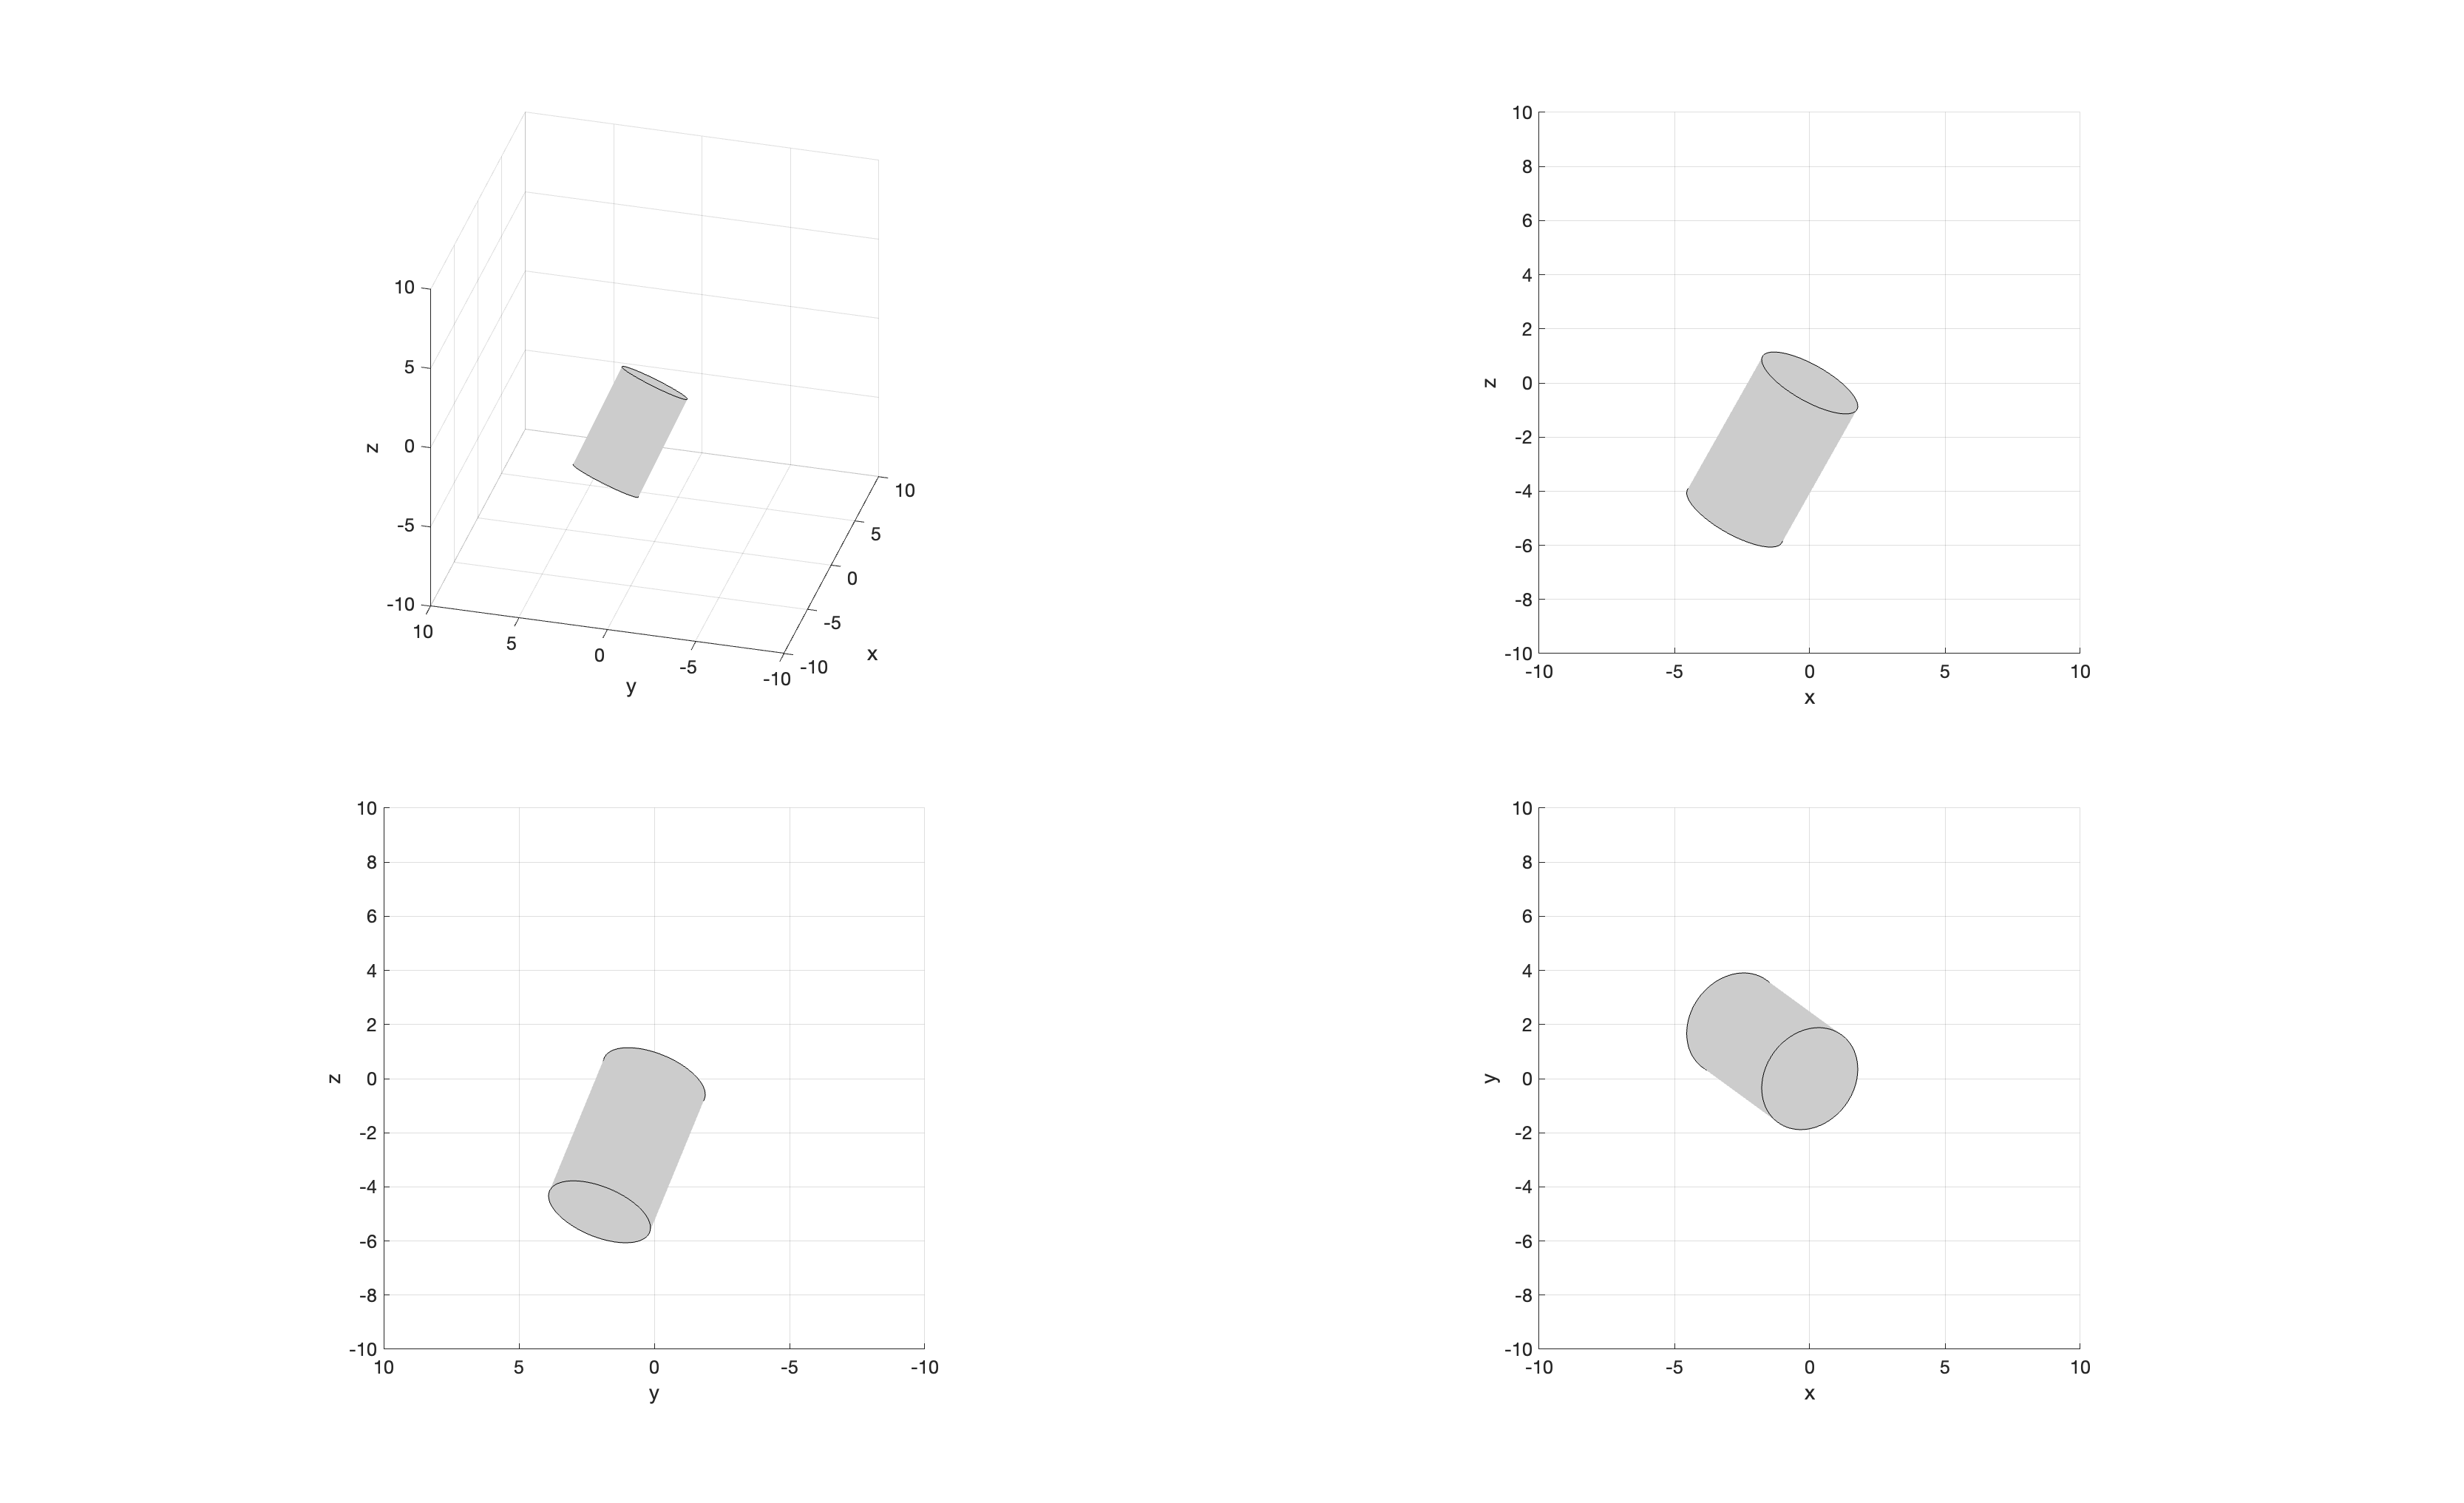
\includegraphics[width=0.45\textwidth]{assets/figure_16.png} & 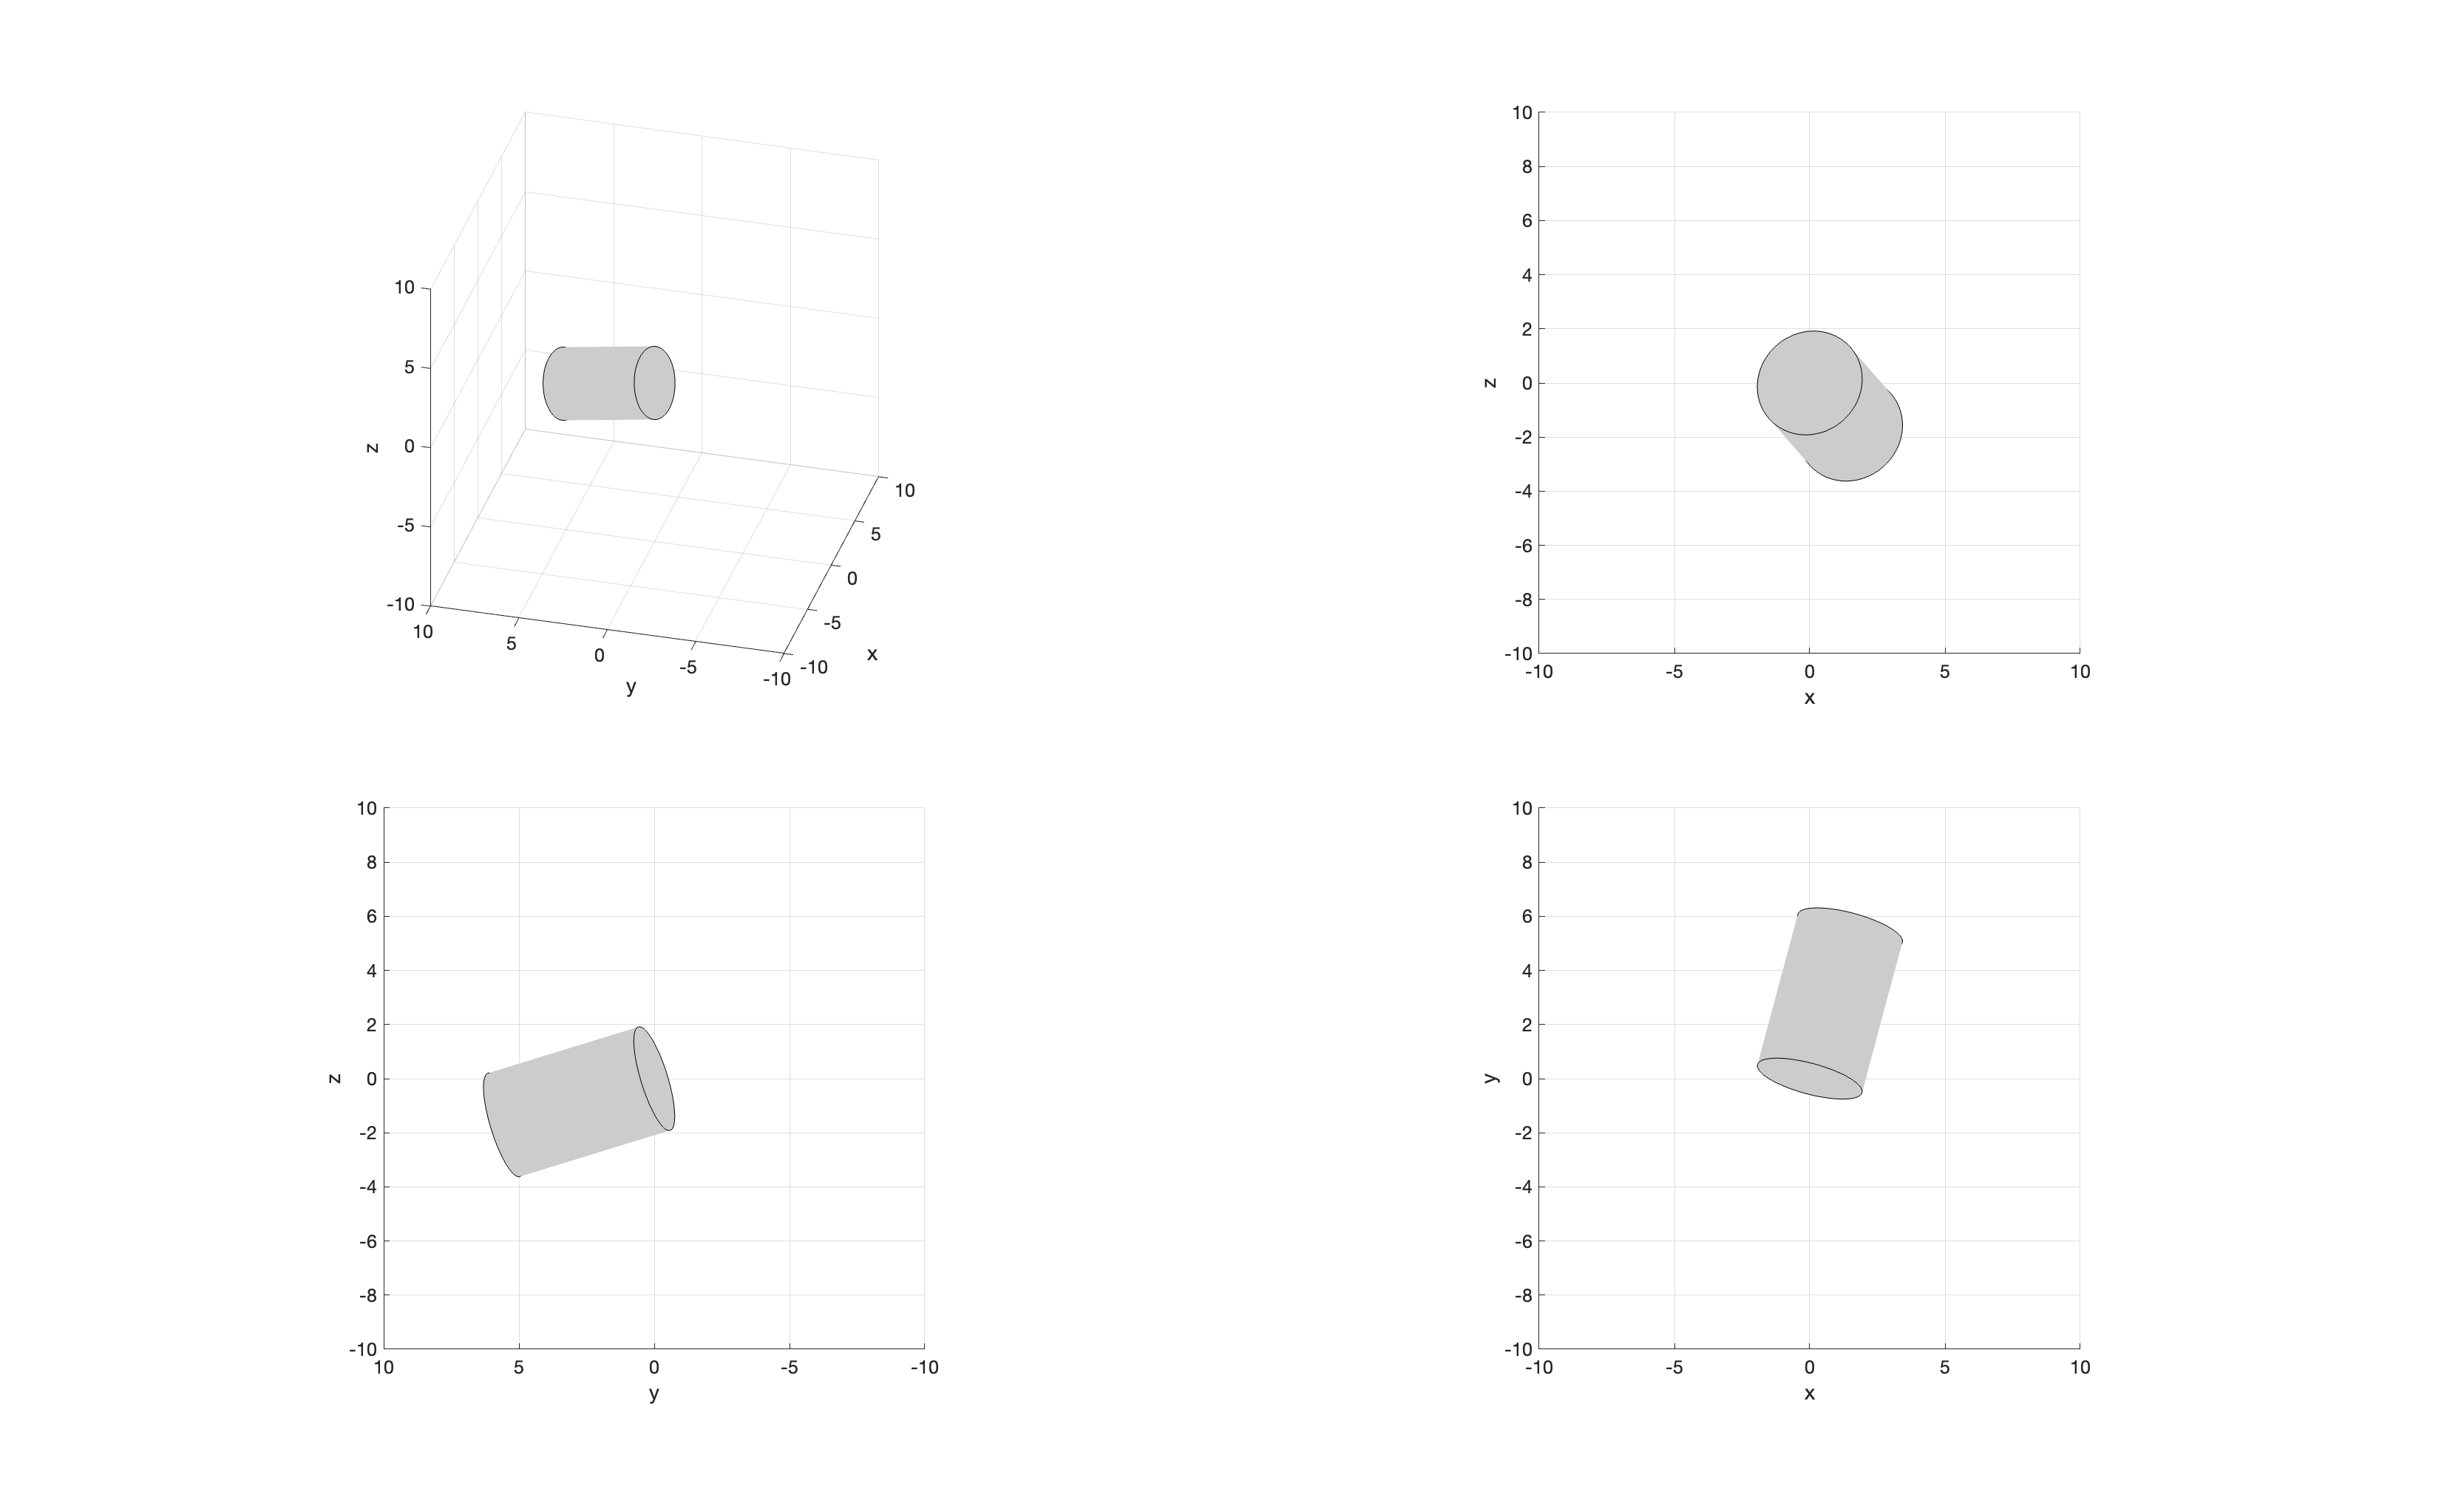
\includegraphics[width=0.45\textwidth]{assets/figure_20.png} \\
    (e) $t = 16$ & (f) $t = 20$ \\
  \end{tabular}
  \caption{Simulation results of the rotation of a cylinder.}
  \label{fig:simulation_results}
\end{figure}
\\
This video can be found at \url{https://youtu.be/vdpJ3pKb_bM}.
\end{document}
